\documentclass[12pt]{article}
\usepackage{amsmath, amssymb}
\allowdisplaybreaks
\usepackage{braket}         % \ket{}, \bra{}
\usepackage{geometry}
\usepackage[UTF8]{ctex}
\usepackage{newtxtext,newtxmath} % Times-like 正文 + 数学字体（PRA/PRL 风格）
\usepackage{graphicx} % 添加图片支持
\usepackage{tikz}     % 添加TikZ支持
\usetikzlibrary{
  arrows.meta,              % 现代箭头（Stealth 等）
  decorations.pathmorphing  % 备用：波浪线等（目前未用）
}

\geometry{a4paper, margin=1in}

% =========================================================
% 全局数学公式样式
% 所有 $...$ 默认使用 displaystyle
% 让 \Omega, \Delta, V_{ij} 更饱满
% =========================================================
\everymath{\displaystyle}

\begin{document}
	
{\centering
\section*{三比特 Toffoli 门非对称激光配置}
}
% TikZ图片
\begin{figure}[h!]
\centering
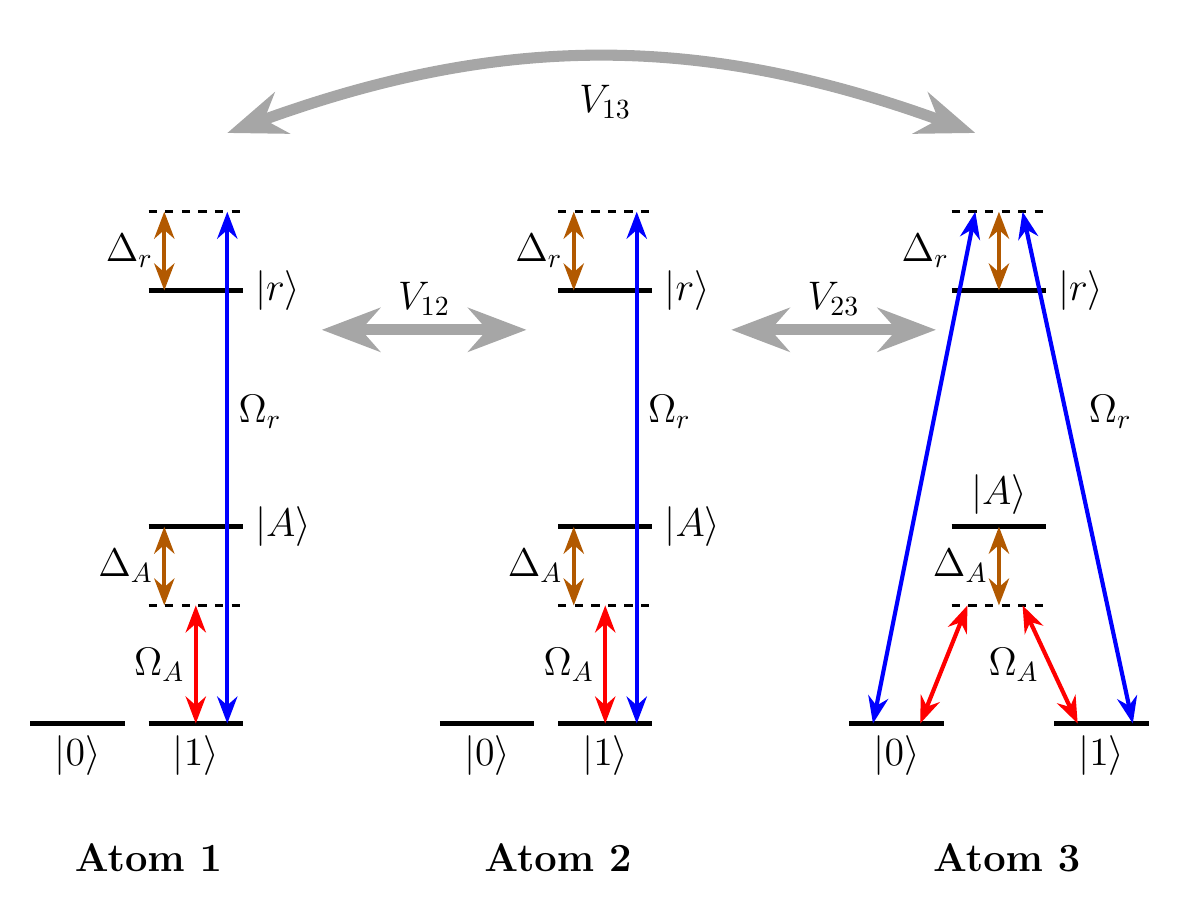
\begin{tikzpicture}[
    % =====================================================
    % 样式定义（只管"画笔属性"，不管几何）
    % =====================================================
    level/.style={
        line width=2pt            % 实能级：较粗实线
    },
    vlevel/.style={
        line width=1.2pt,
        dashed                   % 虚能级：细虚线
    },
    laser/.style={
        <->,
        line width=1.5pt,
        >=Stealth,               % 激光：双向箭头
        draw=blue
    },
    detune/.style={
        <->,
        line width=1.5pt,
        >=Stealth,               % 失谐 Δ：双向箭头
        draw=orange!70!black     % 使用更柔和的橙褐色
    },
    int/.style={
        <->,
        line width=4pt,
        draw=gray!70,
        >=Stealth                % Rydberg 相互作用
    },
    % =====================================================
    % 所有 node 的统一字体设置
    % =====================================================
    every node/.style={
        font=\Large\bfseries,
        text=black
    }
]

% =========================================================
% 全局几何参数（控制整体布局）
% =========================================================

% -------- 三个原子的横向位置 --------
\def\xA{0}        % Atom 1
\def\xB{5.2}      % Atom 2
\def\xC{10.4}     % Atom 3

% -------- 能级高度 --------
\def\yzero{0}     % |0>, |1> 基态
\def\yA{2.5}      % |A> 实能级
\def\yr{5.5}      % |r> 实能级

% -------- 虚能级高度 --------
\def\yAv{1.5}     % |A> 对应虚能级
\def\yrv{6.5}     % |r> 对应虚能级

% =========================================================
% ===================== Atom 1 =============================
% =========================================================

% -------- 基态 |0>, |1> --------
\draw[level] (\xA,\yzero) -- ++(1.2,0)
    node[midway,below] {$\ket{0}$};

\draw[level] (\xA+1.5,\yzero) -- ++(1.2,0)
    node[midway,below] {$\ket{1}$};

% -------- 激发态 |A>, |r> --------
\draw[level] (\xA+1.5,\yA) -- ++(1.2,0)
    node[right] {$\ket{A}$};

\draw[level] (\xA+1.5,\yr) -- ++(1.2,0)
    node[right] {$\ket{r}$};

% -------- 虚能级（激光失谐后的能级） --------
\draw[vlevel] (\xA+1.5,\yAv) -- ++(1.2,0);
\draw[vlevel] (\xA+1.5,\yrv) -- ++(1.2,0);

% -------- 激光驱动 --------
\draw[laser, red]
    (\xA+2.1,\yzero) -- (\xA+2.1,\yAv)
    node[midway,left] {$\Omega_A$};

\draw[laser, blue]
    (\xA+2.5,\yzero) -- (\xA+2.5,\yrv)
    node[midway,right,yshift=20pt] {$\Omega_r$};

% -------- 失谐标注 Δ --------
\draw[detune]
    (\xA+1.7,\yA) -- (\xA+1.7,\yAv)
    node[midway,left] {$\Delta_A$};

\draw[detune]
    (\xA+1.7,\yr) -- (\xA+1.7,\yrv)
    node[midway,left] {$\Delta_r$};

% -------- 原子标签 --------
\node at (\xA+1.5,-1.7) {Atom 1};

% =========================================================
% ===================== Atom 2 =============================
% =========================================================
% （结构与 Atom 1 完全一致，仅横向平移）

\draw[level] (\xB,\yzero) -- ++(1.2,0)
    node[midway,below] {$\ket{0}$};

\draw[level] (\xB+1.5,\yzero) -- ++(1.2,0)
    node[midway,below] {$\ket{1}$};

\draw[level] (\xB+1.5,\yA) -- ++(1.2,0)
    node[right] {$\ket{A}$};

\draw[level] (\xB+1.5,\yr) -- ++(1.2,0)
    node[right] {$\ket{r}$};

\draw[vlevel] (\xB+1.5,\yAv) -- ++(1.2,0);
\draw[vlevel] (\xB+1.5,\yrv) -- ++(1.2,0);

\draw[laser, red]
    (\xB+2.1,\yzero) -- (\xB+2.1,\yAv)
    node[midway,left] {$\Omega_A$};

\draw[laser, blue]
    (\xB+2.5,\yzero) -- (\xB+2.5,\yrv)
    node[midway,right,yshift=20pt] {$\Omega_r$};

\draw[detune]
    (\xB+1.7,\yA) -- (\xB+1.7,\yAv)
    node[midway,left] {$\Delta_A$};

\draw[detune]
    (\xB+1.7,\yr) -- (\xB+1.7,\yrv)
    node[midway,left] {$\Delta_r$};

\node at (\xB+1.5,-1.7) {Atom 2};

% =========================================================
% ===================== Atom 3 (Λ 型) ======================
% =========================================================

% -------- 基态 |0>, |1> --------
\draw[level] (\xC,\yzero) -- ++(1.2,0)
    node[midway,below] {$\ket{0}$};

\draw[level] (\xC+2.6,\yzero) -- ++(1.2,0)
    node[midway,below] {$\ket{1}$};

% -------- 激发态 --------
\draw[level] (\xC+1.3,\yA) -- ++(1.2,0)
    node[midway,above] {$\ket{A}$};

\draw[level] (\xC+1.3,\yr) -- ++(1.2,0)
    node[right] {$\ket{r}$};

% -------- 虚能级 --------
\draw[vlevel] (\xC+1.3,\yAv) -- ++(1.2,0);
\draw[vlevel] (\xC+1.3,\yrv) -- ++(1.2,0);

% -------- Λ 型激光 --------
\draw[laser, blue]
    (\xC+0.3,\yzero) -- (\xC+1.6,\yrv);

\draw[laser, blue]
    (\xC+3.6,\yzero) -- (\xC+2.2,\yrv)
    node[midway,right,yshift=20pt] {$\Omega_r$};

\draw[laser, red]
    (\xC+1.5,\yAv) -- (\xC+0.9,\yzero);

\draw[laser, red]
    (\xC+2.2,\yAv) -- (\xC+2.9,\yzero)
    node[midway,left] {$\Omega_A$};

% -------- 失谐 --------
\draw[detune]
    (\xC+1.9,\yA) -- (\xC+1.9,\yAv)
    node[midway,left] {$\Delta_A$};

\draw[detune]
    (\xC+1.9,\yr) -- (\xC+1.9,\yrv)
    node[midway,left,xshift=-14pt] {$\Delta_r$};

\node at (\xC+2,-1.7) {Atom 3};

% =========================================================
% ================= Rydberg 相互作用 =======================
% =========================================================

% -------- 最近邻相互作用 --------
\draw[int]
    (\xA+3.7,\yrv-1.5) -- (\xB+1.1,\yrv-1.5)
    node[midway,above] {$V_{12}$};

\draw[int]
    (\xB+3.7,\yrv-1.5) -- (\xC+1.1,\yrv-1.5)
    node[midway,above] {$V_{23}$};

% -------- 远程相互作用（弯曲箭头） --------
\draw[int]
    (\xA+2.5,\yrv+1)
    to[out=20, in=160]
    (\xC+1.6,\yrv+1)
    node at (\xB+2.1,\yrv+1.4) {$V_{13}$};

\end{tikzpicture}
\caption{三原子 Toffoli 门能级结构与激光配置示意图。控制原子（Atom1, Atom2）只在 $|1\rangle$ 态有激光耦合，目标原子（Atom3）在 $|0\rangle$ 和 $|1\rangle$ 态均有均匀驱动。图中展示了 $\Omega_r$、$\Omega_A$ 的耦合路径以及 Rydberg 相互作用 $V_{ij}$。}
\end{figure}

	\subsection*{1. 系统设定}
	三个原子：Atom1, Atom2（控制比特），Atom3（目标比特）
	
	每个原子四个能级：
	\begin{itemize}
		\item $|0\rangle, |1\rangle$（基态）
		\item $|A\rangle$（D1 线辅助态）
		\item $|r\rangle$（Rydberg 态）
	\end{itemize}
	
	能量参考：
	\begin{equation}
		\omega_0 = \omega_1 = 0,\quad \omega_A, \omega_r \text{ 为激发态能量}
	\end{equation}
	
	Rydberg 相互作用：
	\begin{equation}
		V_{ij} = C_6 / r_{ij}^6
	\end{equation}
	
	\subsection*{2. 激光配置（全局照射，非对称功能）}
	\begin{center}
		\begin{tabular}{|c|c|c|c|c|}
			\hline
			原子 & 跃迁 & 激光类型 & Rabi 频率 & 失谐（物理） \\
			\hline
			1, 2 & $|1\rangle \leftrightarrow |r\rangle$ & 蓝失谐 & $\Omega_r$ & $+\Delta_r$ \\
			1, 2 & $|1\rangle \leftrightarrow |A\rangle$ & 红失谐 & $\Omega_A$ & $-\Delta_A$ \\
			3 & $|0\rangle \leftrightarrow |r\rangle$ & 蓝失谐 & $\Omega_r$ & $+\Delta_r$ \\
			3 & $|1\rangle \leftrightarrow |r\rangle$ & 蓝失谐 & $\Omega_r$ & $+\Delta_r$ \\
			3 & $|0\rangle \leftrightarrow |A\rangle$ & 红失谐 & $\Omega_A$ & $-\Delta_A$ \\
			3 & $|1\rangle \leftrightarrow |A\rangle$ & 红失谐 & $\Omega_A$ & $-\Delta_A$ \\
			\hline
		\end{tabular}
	\end{center}
	
	\textbf{物理含义}：
	\begin{itemize}
		\item 控制原子：只在 $|1\rangle$ 时有激光耦合
		\item 目标原子：不论 $|0\rangle$ 或 $|1\rangle$ 均被均匀驱动
	\end{itemize}
	
	\subsection*{3. 相互作用绘景下的哈密顿量（分原子写出）}
	我们选择自由哈密顿量为：
	\begin{equation}
		H_0 = \sum_{j=1}^3 \left( \omega_A |A\rangle_j\langle A| + \omega_r |r\rangle_j\langle r| \right)
	\end{equation}
	定义变换算符：
	\begin{equation}
		U_0(t) = e^{-iH_0 t}
	\end{equation}
	
	\subsubsection*{原子1（控制原子）在相互作用绘景中}
	原哈密顿量：
	\begin{equation}
		H_1(t) = H_{\text{energy}}^{(1)} + \frac{\Omega_r}{2} e^{i(\omega_r + \Delta_r)t} |1\rangle_1\langle r| + \frac{\Omega_A}{2} e^{i(\omega_A - \Delta_A)t} |1\rangle_1\langle A| + \text{h.c.}
	\end{equation}
	变换到相互作用绘景（旋转掉 $H_0$）：
	\begin{equation}
		\begin{aligned}
			H_{I,1}(t) &= U_0^\dagger(t) H_1(t) U_0(t) - i U_0^\dagger(t) \frac{dU_0(t)}{dt} \\
			&= \frac{\Omega_r}{2} e^{i\Delta_r t} |1\rangle_1\langle r| + \frac{\Omega_A}{2} e^{-i\Delta_A t} |1\rangle_1\langle A| + \text{h.c.}
		\end{aligned}
	\end{equation}
	
	\subsubsection*{原子2（控制原子）在相互作用绘景中}
	类似地：
	\begin{equation}
		H_{I,2}(t) = \frac{\Omega_r}{2} e^{i\Delta_r t} |1\rangle_2\langle r| + \frac{\Omega_A}{2} e^{-i\Delta_A t} |1\rangle_2\langle A| + \text{h.c.}
	\end{equation}
	
	\subsubsection*{原子3（目标原子）在相互作用绘景中}
	\begin{equation}
		H_{I,3}(t) = \frac{\Omega_r}{2} e^{i\Delta_r t} \big( |0\rangle_3\langle r| + |1\rangle_3\langle r| \big) + \frac{\Omega_A}{2} e^{-i\Delta_A t} \big( |0\rangle_3\langle A| + |1\rangle_3\langle A| \big) + \text{h.c.}
	\end{equation}
	
	\subsection*{4. 简化模型：忽略 $|A\rangle$ 通道（分原子写出）}
	为了简化计算，类比于 CNOT 门，我们知道状态 $|r\rangle$ 与状态 $|A\rangle$ 之间的拉曼跃迁过程被抑制。因此，由具有拉比频率 $\Omega_r$ 和 $\Omega_A$ 的色散激光诱导的有效哈密顿量可独立考虑。我们先不考虑中间能级 $|A\rangle$，将单个原子哈密顿量中 $|A\rangle$ 的过程不写。
	
	\subsubsection*{原子1（控制原子）在简化模型中}
	\begin{equation}
		H_{I,1}^{\text{(sim)}}(t) = \frac{\Omega_r}{2} e^{i\Delta_r t} |1\rangle_1\langle r| + \text{h.c.}
	\end{equation}
	
	\subsubsection*{原子2（控制原子）在简化模型中}
	\begin{equation}
		H_{I,2}^{\text{(sim)}}(t) = \frac{\Omega_r}{2} e^{i\Delta_r t} |1\rangle_2\langle r| + \text{h.c.}
	\end{equation}
	
	\subsubsection*{原子3（目标原子）在简化模型中}
	\begin{equation}
		H_{I,3}^{\text{(sim)}}(t) = \frac{\Omega_r}{2} e^{i\Delta_r t} \big( |0\rangle_3\langle r| + |1\rangle_3\langle r| \big) + \text{h.c.}
	\end{equation}
	
	\subsubsection*{系统总哈密顿量（简化模型）}
	\begin{equation}
		\begin{aligned}
			H_I^{\text{(sim)}}(t) &= H_{I,1}^{\text{(sim)}}(t) \otimes I_2 \otimes I_3 \\
			&+ I_1 \otimes H_{I,2}^{\text{(sim)}}(t) \otimes I_3 \\
			&+ I_1 \otimes I_2 \otimes H_{I,3}^{\text{(sim)}}(t) \\
			&+ \sum_{i<j} V_{ij} |rr\rangle\langle rr|_{ij}
		\end{aligned}
	\end{equation}
	
	\subsection*{5. 第二次旋转变换}
	定义新的变换矩阵，根据 $H_R = H_v + H_0$，其中 $H_v$ 是 Rydberg 相互作用项，$H_0$ 是失谐项：
	\begin{equation}
		U(t) = \exp\left[-i \left( \sum_{i<j} V_{ij} |rr\rangle\langle rr|_{ij} + \Delta_r \sum_{j=1}^3 |r\rangle_j\langle r| \right) t \right]
	\end{equation}
	新相互作用绘景中的哈密顿量为：
	\begin{equation}
		H_{\text{rot}}(t) = U^\dagger(t) H_I^{\text{(sim)}}(t) U(t) - i U^\dagger(t) \frac{dU(t)}{dt}
	\end{equation}
	在 $V = \Delta_r$ 的条件下，得到：
	\begin{equation}
		\begin{aligned}
			H(t) = &\frac{\Omega_r}{2}e^{i\Delta_r t}\Big[|000\rangle\langle 00r| + |001\rangle\langle 00r| + |010\rangle\langle 01r| + |010\rangle\langle 0r0| \\
			&\quad + |011\rangle\langle 01r| + |011\rangle\langle 0r1| + |0rr\rangle\langle 01r| + |0rr\rangle\langle 0r0| + |0rr\rangle\langle 0r1| \\
			&\quad + |100\rangle\langle 10r| + |100\rangle\langle r00| + |101\rangle\langle 10r| + |101\rangle\langle r01| \\
			&\quad + |110\rangle\langle 11r| + |110\rangle\langle 1r0| + |110\rangle\langle r10| + |111\rangle\langle 11r| \\
			&\quad + |111\rangle\langle 1r1| + |111\rangle\langle r11| + |1rr\rangle\langle 11r| + |1rr\rangle\langle 1r0| \\
			&\quad + |1rr\rangle\langle 1r1| + |r0r\rangle\langle 10r| + |r0r\rangle\langle r00| + |r0r\rangle\langle r01| \\
			&\quad + |r1r\rangle\langle 11r| + |r1r\rangle\langle r10| + |r1r\rangle\langle r11| + |rr0\rangle\langle 1rr| \\
			&\quad + |rr0\rangle\langle r1r| + |rr1\rangle\langle 1rr| + |rr1\rangle\langle r1r|\Big] + \mathrm{H.c.} \\
			&\quad + \frac{\Omega_r}{2}\Big[|1rr\rangle\langle rrr| + |r1r\rangle\langle rrr| + |rr0\rangle\langle rrr| + |rr1\rangle\langle rrr| + \mathrm{H.c.}\Big] \\
			&\quad - \Delta_r\Big[|0rr\rangle\langle 0rr| + |1rr\rangle\langle 1rr| + |r0r\rangle\langle r0r| + |r1r\rangle\langle r1r| \\
			&\quad + |rr0\rangle\langle rr0| + |rr1\rangle\langle rr1|\Big]
		\end{aligned}
	\end{equation}
	
	\subsection*{6. 高频近似与有效哈密顿量}
	接着进行高频近似，我们发现无法直接得出有效哈密顿量，因此继续进行相互作用绘景变换。选取新的 $U$ 矩阵继续做 $U = e^{-i H_0 t}$ 的旋转，相互作用绘景，接着进行高频近似，消去单激发与双激发态，和无效耦合过程，忽略高频震荡项，我们可以得到：
	\begin{equation}
		\begin{aligned}
			H_{\text{eff}} = &\frac{\Omega_r^2}{4\Delta_r} \big( |000\rangle\langle 000| + |001\rangle\langle 001| \big) \\
			&+ \frac{\Omega_r^2}{2\Delta_r} \big( |010\rangle\langle 010| + |011\rangle\langle 011| + |100\rangle\langle 100| + |101\rangle\langle 101| \big) \\
			&+ \frac{3\Omega_r^2}{4\Delta_r} \big( |110\rangle\langle 110| + |111\rangle\langle 111| \big) \\
			&+ \frac{\Omega_r^2}{\Delta_r} |RRR\rangle\langle RRR| \\
			&+ \frac{3\Omega_r^3}{4\Delta_r^2} \big( |110\rangle\langle RRR| + |111\rangle\langle RRR| + \mathrm{H.c.} \big)
		\end{aligned}
	\end{equation}
	
	\subsection*{7. 引入中间能级 $|A\rangle$ 抵消对角项}
	这里与 CNOT 门一致，我们引入中间能级 $|A\rangle$ 以抵消对角项（斯塔克位移）。对应激光参数为：
	\begin{equation}
		\Omega_A \quad (\text{Rabi 频率}), \quad \Delta_A \quad (\text{失谐})
	\end{equation}
	通过类似的旋转变换、高频近似和微扰论，可以得到包含 $|A\rangle$ 能级的有效哈密顿量，用于抵消由 $|r\rangle$ 能级引起的对角斯塔克位移。
	
	\subsubsection*{通过中间能级 $|A\rangle$ 耦合的有效哈密顿量}
	基矢顺序：$\{|000\rangle, |001\rangle, |010\rangle, |011\rangle, |100\rangle, |101\rangle, |110\rangle, |111\rangle, |RRR\rangle\}$：
	\begin{equation}
		\begin{aligned}
			H_2 = &-\frac{\Omega_A^2}{4\Delta_A} \big( |000\rangle\langle 000| + |001\rangle\langle 001| \big) \\
			&-\frac{\Omega_A^2}{2\Delta_A} \big( |010\rangle\langle 010| + |011\rangle\langle 011| + |100\rangle\langle 100| + |101\rangle\langle 101| \big) \\
			&-\frac{3\Omega_A^2}{4\Delta_A} \big( |110\rangle\langle 110| + |111\rangle\langle 111| \big)
		\end{aligned}
	\end{equation}
	当满足条件：
	\begin{equation}
		\frac{\Omega_r^2}{\Delta_r} = \frac{\Omega_A^2}{\Delta_A}
	\end{equation}
	时，正负位移相互抵消，总对角项为零。
	
	总有效哈密顿量为：
	\begin{equation}
		H_{\text{EFF}} = H_{\text{eff}} + H_2
	\end{equation}
	简化后得到：
	\begin{equation}
		\begin{aligned}
			H_{\text{EFF}} = &\frac{3\Omega_r^3}{4\Delta_r^2} \big( |110\rangle\langle RRR| + |111\rangle\langle RRR| +\mathrm{H.c.} \big) \\
			&+ \frac{\Omega_r^2}{\Delta_r} |RRR\rangle\langle RRR|
		\end{aligned}
	\end{equation}
	
	\subsection*{8. 修正的反封锁条件与最终哈密顿量}
	令 Rydberg 相互作用满足修正的反封锁条件：
	\begin{equation}
		V = \Delta_r - \frac{\Omega_r^2}{3\Delta_r}
	\end{equation}
	此时 $|RRR\rangle$ 的斯塔克位移被精确抵消。最终哈密顿量为：
	\begin{equation}
		\begin{aligned}
			H_{\text{EFF}} = \frac{3\Omega_r^3}{4\Delta_r^2} \big( |110\rangle\langle RRR| + |111\rangle\langle RRR| +\mathrm{H.c.} \big)
		\end{aligned}
	\end{equation}
	
	\subsection*{9. Toffoli 门的实现}
	在时间
	\begin{equation}
		t_g = \frac{2\sqrt{2}\pi\Delta_r^2}{3\Omega_r^3}
	\end{equation}
	下，得到矩阵
	\begin{equation}
		U(t_g) = 
		\begin{pmatrix}
			1 & 0 & 0 & 0 & 0 & 0 & 0 & 0 & 0 \\
			0 & 1 & 0 & 0 & 0 & 0 & 0 & 0 & 0 \\
			0 & 0 & 1 & 0 & 0 & 0 & 0 & 0 & 0 \\
			0 & 0 & 0 & 1 & 0 & 0 & 0 & 0 & 0 \\
			0 & 0 & 0 & 0 & 1 & 0 & 0 & 0 & 0 \\
			0 & 0 & 0 & 0 & 0 & 1 & 0 & 0 & 0 \\
			0 & 0 & 0 & 0 & 0 & 0 & 0 & -1 & 0 \\
			0 & 0 & 0 & 0 & 0 & 0 & -1 & 0 & 0 \\
			0 & 0 & 0 & 0 & 0 & 0 & 0 & 0 & -1
		\end{pmatrix}
	\end{equation}
	消去 $|RRR\rangle$ 态（第9行第9列）后，得到在计算基 $\{|000\rangle, |001\rangle, |010\rangle, |011\rangle, |100\rangle, |101\rangle, |110\rangle, |111\rangle\}$ 上的算符：
	\begin{equation}
		U_{\text{Toffoli}} = 
		\begin{pmatrix}
			1 & 0 & 0 & 0 & 0 & 0 & 0 & 0 \\
			0 & 1 & 0 & 0 & 0 & 0 & 0 & 0 \\
			0 & 0 & 1 & 0 & 0 & 0 & 0 & 0 \\
			0 & 0 & 0 & 1 & 0 & 0 & 0 & 0 \\
			0 & 0 & 0 & 0 & 1 & 0 & 0 & 0 \\
			0 & 0 & 0 & 0 & 0 & 1 & 0 & 0 \\
			0 & 0 & 0 & 0 & 0 & 0 & 0 & -1 \\
			0 & 0 & 0 & 0 & 0 & 0 & -1 & 0
		\end{pmatrix}
	\end{equation}
	该矩阵对应 Toffoli 门（CCNOT）操作。
	
\end{document}
